\begin{technical}
{\Large\textbf{Mathematical Foundations of the Banach-Tarski Paradox}}

\textbf{Overview.}  
The Banach-Tarski paradox states that a three-dimensional ball can be partitioned into a finite number of disjoint subsets and reassembled, via rigid motions alone, into two balls identical to the original. This result contradicts classical volume conservation but arises within set theory under the Axiom of Choice. The construction depends on the existence of non-measurable sets and the group-theoretic properties of rotations in \(\mathbb{R}^3\), particularly the presence of a free subgroup within \(\mathrm{SO}(3)\).

\textbf{Structure of the Proof.}  
The proof follows four main steps:
\begin{itemize}[leftmargin=*]
    \item \textbf{Step 1: Paradoxical Decomposition of a Free Group.}  
    The free group \( F_2 = \langle a, b \rangle \), generated by two elements with no defining relations other than identity, can be partitioned into two subsets that are each equivalent to the whole under group multiplication. This self-replicating structure is fundamental to the paradox.
    
    \item \textbf{Step 2: Embedding \( F_2 \) into \(\mathrm{SO}(3)\).}  
    A subgroup of \(\mathrm{SO}(3)\) can be found that behaves like \( F_2 \). Two properly chosen rotations \( A \) and \( B \), about different axes, generate a subgroup where no nontrivial combination of \( A \) and \( B \) (except the identity) returns a point to its original location. This free subgroup allows a similar paradoxical decomposition to be applied to rotations in three-dimensional space.

    \item \textbf{Step 3: Partitioning the Sphere.}  
    The unit sphere \( S^2 \) is decomposed into orbits under the action of this free subgroup. The Axiom of Choice is used to select a single representative from each orbit, forming a non-measurable set. Applying the same group action, these pieces can be rearranged into two distinct copies of the original sphere.

    \item \textbf{Step 4: Extending to the Ball.} 
    The paradoxical decomposition of \( S^2 \) extends to the full three-dimensional ball by associating each point on the sphere with a radial segment. Each segment inherits the same paradoxical partitioning, allowing the entire solid ball to be duplicated.
\end{itemize}
\columnbreak
\textbf{Free Groups, the Cayley Graph, and Self-Similarity.}  
The underlying structure of \( F_2 = \langle a, b \rangle \) can be visualized through its \emph{Cayley graph}, an infinite branching tree where each node represents a group element, and edges correspond to multiplication by \( a \), \( a^{-1} \), \( b \), or \( b^{-1} \). Each branch of the tree contains a subgraph isomorphic to the entire structure, demonstrating the key self-replicating property. This same self-similarity is leveraged in the Banach-Tarski construction: just as subgraphs of the Cayley graph replicate the whole, subsets of the sphere can be transformed into complete copies under the action of a free subgroup of \(\mathrm{SO}(3)\).

\begin{center}
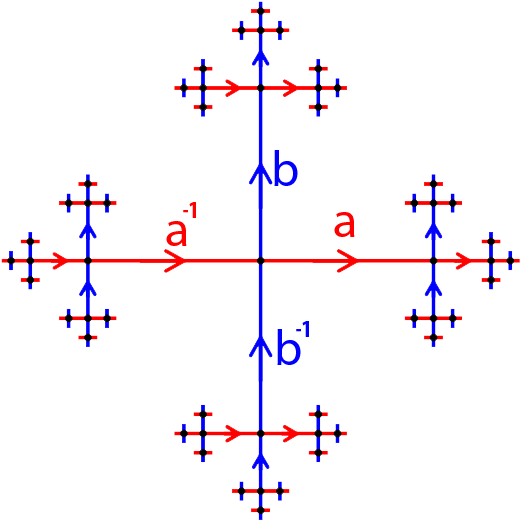
\includegraphics[width=0.4\textwidth]{01_BanachTarskiParadox/F2_Cayley_Graph_tp.png}

\vspace{0.5em}
\small
\textbf{Figure:} Cayley graph of \( F_2 = \langle a, b \rangle \). Each node corresponds to a group element, and each directed edge corresponds to multiplication by \( a \), \( a^{-1} \), \( b \), or \( b^{-1} \). The infinite tree structure reflects the group's free, non-relational nature.
\end{center}


\vspace{0.5em}
\noindent\textbf{References}\\
Banach, S. \& Tarski, A. (1924). Sur la décomposition des ensembles de points en parties respectivement congruentes. \emph{Fund. Math.}, \textbf{6}, 244-277.\\
Wagon, S. (1993). \emph{The Banach-Tarski Paradox}. Cambridge University Press.\\
\end{technical}
